\documentclass[12pt]{report}
\usepackage[utf8]{inputenc}
\usepackage[margin=1.2in]{geometry}
\usepackage{graphicx}
\usepackage{float}
\usepackage{subcaption}
\usepackage{amsmath}
\usepackage{amssymb}
\usepackage{ulem}
\usepackage{bm}
\usepackage{framed}
\usepackage{xcolor}
\usepackage{ragged2e}
\usepackage{color}
\usepackage{soul}
\usepackage{cancel}
\graphicspath{ {images/} }
\setlength{\parskip}{1em}
\allowdisplaybreaks


\usepackage{titling}
\newcommand{\subtitle}[1]{%
	\posttitle{%
		\par\end{center}
	\begin{center}\large#1\end{center}
	\vskip0.5em}%
}

\newenvironment{blueframed}[1][blue]
{\def\FrameCommand{\fboxsep=\FrameSep\fcolorbox{#1}{white}}%
\MakeFramed {\advance\hsize-\width \FrameRestore}}
{\endMakeFramed}

\newenvironment{spmatrix}[1]
{\def\mysubscript{#1}\mathop\bgroup\begin{bmatrix}}
{\end{bmatrix}\egroup_{\textstyle\mathstrut\mysubscript}}

\title{Tutorial 10}
\subtitle
{
\textbf{keywords}: grouped data, variance, error, heteroskedasticity, homoskedasticity, residual plots, Breusch-Pagan test, inference, efficiency, Weighted Least Squares estimator

\textbf{estimated reading time}: 32 minutes
}
\author{Quang Bui}
\date{May 7, 2018}

\begin{document}

\maketitle

\section*{Question 1}
\noindent EViews workfile: \textit{Tobin.wf1}

\noindent \textit{Tobin.wf1} contains data from the US 1941 Family Budget Survey data set. We have information about 37 family groups. Each group is based on number of people in the family (1,2,3,4,5+) and their income range (0-500, 500-1000, 1000-1500, 1500-2000, 2000-2500, 2500-3000, 3000-4000, 4000+). Information about each family group is held in the following variables:
\begin{align*}
food &- average\ expenditure\ on\ food\ for\ a\ particular\ group\ (\$) \\
inc &- average\ income\ for\ a\ particular\ group\ (\$) \\
nf &- average\ number\ of\ people\ in\ family\ for\ a\ particular\ group \\
ng &- number\ of\ families\ in\ each\ group
\end{align*}
\vspace{-\baselineskip}
%%%%%%%%%% TABLE OBJECT %%%%%%%%%%
\begin{table}[H]
	\centering
	\begin{tabular}{lrrrr}
		\multicolumn{1}{c}{}&\multicolumn{1}{r}{FOOD}&\multicolumn{1}{r}{INC}&\multicolumn{1}{r}{NF}&\multicolumn{1}{r}{NG}\\
		\multicolumn{1}{c}{1}&\multicolumn{1}{r}{$210$}&\multicolumn{1}{r}{$421$}&\multicolumn{1}{r}{$1$}&\multicolumn{1}{r}{$59$}\\
		\multicolumn{1}{c}{2}&\multicolumn{1}{r}{$301$}&\multicolumn{1}{r}{$824$}&\multicolumn{1}{r}{$1$}&\multicolumn{1}{r}{$71$}\\
		\multicolumn{1}{c}{3}&\multicolumn{1}{r}{$369$}&\multicolumn{1}{r}{$1287$}&\multicolumn{1}{r}{$1$}&\multicolumn{1}{r}{$40$}\\
		\multicolumn{1}{c}{4}&\multicolumn{1}{r}{$433$}&\multicolumn{1}{r}{$1703$}&\multicolumn{1}{r}{$1$}&\multicolumn{1}{r}{$18$}\\
		\multicolumn{1}{c}{5}&\multicolumn{1}{r}{$506$}&\multicolumn{1}{r}{$2150$}&\multicolumn{1}{r}{$1$}&\multicolumn{1}{r}{$11$}\\
		\multicolumn{1}{c}{6}&\multicolumn{1}{r}{$621$}&\multicolumn{1}{r}{$2655$}&\multicolumn{1}{r}{$1$}&\multicolumn{1}{r}{$6$}\\
		\multicolumn{1}{c}{7}&\multicolumn{1}{r}{$239$}&\multicolumn{1}{r}{$520$}&\multicolumn{1}{r}{$2$}&\multicolumn{1}{r}{$29$}\\
		\multicolumn{1}{c}{8}&\multicolumn{1}{r}{$319$}&\multicolumn{1}{r}{$869$}&\multicolumn{1}{r}{$2$}&\multicolumn{1}{r}{$54$}\\
		\multicolumn{1}{c}{9}&\multicolumn{1}{r}{$454$}&\multicolumn{1}{r}{$1379$}&\multicolumn{1}{r}{$2$}&\multicolumn{1}{r}{$67$}\\
		\multicolumn{1}{c}{10}&\multicolumn{1}{r}{$517$}&\multicolumn{1}{r}{$1846$}&\multicolumn{1}{r}{$2$}&\multicolumn{1}{r}{$58$}\\
	\end{tabular}
	\caption{Data on \textit{average food expenditure}, \textit{average income}, \textit{average family size} and \textit{number of families in the group} for the first 10 family groups in our data set of 37 family groups.}
	%\label{tab:}
\end{table}
\vspace{-\baselineskip}
\begin{itemize}
	\item Family group number 1 contains 59 families ($ng = 59$), spends \$210 on food on average ($food = 210$), has an average income of \$421 ($inc = 421$) and an average family size of 1 member ($nf = 1$). This family group represents familes with 1 family member with an income range of \$0-500.
	\item Family group number 2 contains 71 families ($ng = 71$), spends \$301 on food on average ($food = 301$), has an average income of \$824 ($inc = 824$) and an average family size of 1 member ($nf = 1$). This family group represents familes with 1 family member with an income range of \$500-1000.
	\item etc.
\end{itemize}

\noindent \textcolor{red}
{
	(a) Suppose that food consumption is related to family income and number of people in each family according to the following model.
	$$food_i = \beta_0 + \beta_1inc_i + \beta_2nf_i + u_i$$
	Argue that even if the above model is a fair description of each family's demand for food and all Gauss-Markov assumptions are satisfied for this model, we may expect heteroskedastic errors when we estimate the model using \textbf{group averaged data}.	
}

\noindent If we estimate the model with data on \textbf{individual families} such that,
\begin{align*}
food_i &- i^{th}\ family's\ food\ expenditure\ \\
inc_i &- i^{th}\ family's\ income\ \\
nf_i &- i^{th}\ family's\ number\ of\ family\ members\
\end{align*}
\noindent then we will assume that the errors are homoskedastic (although this assumption is not reasonable, we make this assumption to validate today's exercise). If instead, we estimate the model using \textbf{group averaged data} then it would be very unreasonable to assume homoskedastic errors. Why?
\justify
\begin{blueframed}
	\textcolor{blue}{\textbf{Background}}
	\vspace{-\baselineskip}
	\justify
	\textcolor{blue}{\underline{Homoskedasticity}}
	
	\noindent \textcolor{blue}
	{
		For a model that is linear in parameters without perfect collinearity, if the assumption for unbiasedness (zero conditional mean) holds, $$E(\textbf{\textit{u}}|\textbf{\textit{X}}) = \textbf{0}$$ the OLS estimator becomes an unbiased linear estimator. If, in addition to the unbiasedness assumption, the errors are serially uncorrelated and homoskedastic, \begin{align*}
		Var(\textbf{\textit{u}}|\textbf{\textit{X}}) &= \sigma^2\textbf{\textit{I}}_n \\
		&=\begin{bmatrix}
		\sigma^2 & 0 & \dots & 0 \\
		0 & \sigma^2 & \vdots & 0 \\
		\vdots & \dots & \ddots & \dots \\
		0 & 0 & \dots & \sigma^2
		\end{bmatrix}
		\end{align*} $$(off\ diagonal\ elements = 0 \implies unserially\ uncorrelated\ errors)$$ $$(diagonal\ elements = \sigma^2 \implies homoskedastic\ errors)$$ then the OLS estimator becomes the \textit{most efficient linear unbiased estimator}. 
	}
\end{blueframed}
\begin{blueframed}
	\noindent \textcolor{blue}
	{
		Homoskedasticity errors - the variance of the error is constant i.e. the variance is fixed across all observations (if the error does not vary differently across different observations then it is constant regardless of the value of $x$).
		$$Var(u_i|inc_i,nf_i) = \sigma^2$$
		Heteroskedasticity errors - the variance of the error is not constant.
		$$Var(u_i|inc_i,nf_i) \neq \sigma^2$$
		Since $\beta_0$, $\beta_1$ and $\beta_2$ are constants and $inc_i$ and $nf_i$ are known (we have conditioned on $inc_i$ and $nf_i$),
		\begin{align*}
		Var(food_i|inc_i,nf_i) &= Var(\beta_0 + \beta_1inc_i + \beta_2nf_i + u_i|inc_i,nf_i) \\ 
		&= Var(u_i|inc_i,nf_i)
		\end{align*}
		We expect the variability of a family group's average food expenditure, $$Var(food_i|inc_i,nf_i)$$ to depend on the number of families in the group, $$Var(food_i|inc_i,nf_i) = f(ng_i)$$ i.e. we expect average food expenditure to vary less across family groups with many families than family groups with few families, $$Var(food_i|inc_i,nf_i) = \dfrac{\sigma^2}{ng_i} \neq \sigma^2$$ an inverse relationship. \\ \\ 
		Since, $$Var(food_i|inc_i,nf_i) = Var(u_i|inc_i,nf_i)$$ when the variance of the dependent variable is not constant, the variance of the error will not be constant i.e. the error is heteroskedastic.
	}
\end{blueframed}
\noindent \uline{Sampling variability of sample mean}

\noindent Let $X$ be a random variable with variance equal to $\sigma^2$,
$$Var(X) = \sigma^2$$
\noindent For $n$ random variables $X_1, X_2, \dots, X_n$, that are identically distributed to $X$ and independent of each other, a draw from each random variable $X_1, X_2, \dots, X_n$ gives $n$ independent observations i.e. a random sample of size $n$. Since each random variable is identical in distribution, the variance of each random variable equal to $\sigma^2$,
$$Var(X_1) = Var(X_2) = \dots = Var(X_n) = \sigma^2$$
\noindent Since, $$\bar{X} = \dfrac{X_1 + X_2 + \dots + X_n}{n}$$
\noindent if follows that $\bar{X}$ is a random variable that depends on $X_1$, $X_2$ $\dots$ $X_n$ and sample size $n$ and is \textit{subject to sampling variability}. For example, using a sample size of $5$ to apply seven repeated sampling, we obtain the following seven $\bar{X}$,
\begin{figure}[H]
	\centering
	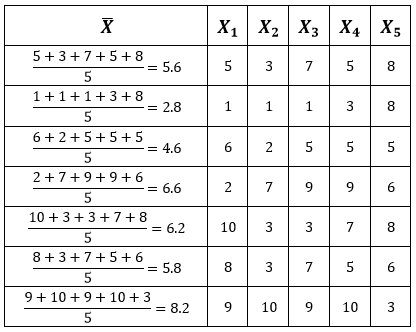
\includegraphics{q1_7}
\end{figure}
\vspace{-\baselineskip}
$$(can\ you\ guess\ the\ distribution\ of\ \textit{X}?)$$ $$(what\ about\ the\ distribution\ of\ \bar{X}?)$$ 

\noindent The sampling variability of $\bar{X}$ is given by,
\begin{align*}
Var(\bar{X}) &= Var\Big(\dfrac{X_1 + X_2 + \dots + X_n}{n}\Big) \\
&= \dfrac{1}{n^2}Var(X_1 + X_2 + \dots + X_n) \\
&= \dfrac{1}{n^2}\Big(Var(X_1) + Var(X_2) + \dots + Var(X_n)\Big) + 0 + 0 + \dots + 0 \\
& (Covariance\ between\ independent\ random\ variables\ equals\ to\ 0) \\
&= \dfrac{1}{n^2}(\sigma^2 + \sigma^2 + \dots + \sigma^2) \\
&= \dfrac{1}{n^2}(n \times \sigma^2) \\ 
&= \dfrac{\sigma^2}{n}
\end{align*}
\noindent which tells us that the sampling variability of $\bar{X}$ equals to the variance of $X$ divided by the sample size. The greater the sample size used to obtain $\bar{X}$, the less sampling variability $\bar{X}$ will have.


\noindent \textcolor{red}
{
	Show that it is logical to expect that variance of errors are inversely proportional to the number of familes in each group i.e. $Var(u_i|inc_i,nf_i) = \dfrac{\sigma^2}{ng_i}$.
}
$$(See\ above)$$
\noindent Assume that, if the model were estimated using \textbf{individual family data}, the errors are homoskedastic so that the variance of family food expenditure equals to $\sigma^2$,
$$Var(food^*_i|inc^*_i, nf^*_i) = Var(u^*_i|inc^*_i,nf^*_i) = \sigma^2$$ 
\noindent Since $food_i$ represents the average food expenditure for the $i^{th}$ family group, $$food_i = \overline{food_i^*}$$ the variance of the average food expenditure for the $i^{th}$ family group is based on the number of families in the $i^{th}$ group i.e. $ng_i$ families. More specifically, the variance of the $i^{th}$ group's average food expenditure equals to the variance of family food expenditure divided by $ng_i$,
\begin{align*}
Var(food_i|inc_i,nf_i) &= \dfrac{\sigma^2}{ng_i} \\
&= Var(u_i|inc_i,nf_i)
\end{align*}
\noindent Since the number of families in each group is not constant i.e. $ng_i$ is not constant, the error is heteroskedastic i.e. the variance of the error when the model is estimated with \textbf{group average data} depends on the number of families in each group.

\noindent \textcolor{red}
{
	(b) If errors are heteroskedastic, would OLS be unbiased? Explain.
}

\noindent The condition for homoskedastic errors is not required for the OLS estimator to be unbiased, therefore, as long as the assumptions for unbiasedness holds, the OLS estimator will still be unbiased even when errors are heteroskedastic.


\noindent \textcolor{red}
{
	(c) Estimate the model using OLS. Then explore visually if the error variance is likely to be inversely proportional to the number of families in each group $(ng)$, and then formally test the hypothesis of no heteroskedasticity against the alternative that, $$Var(u_i|inc_i,nf_i)=\dfrac{\sigma^2}{ng_i}$$
	Hint: Breusch-Pagan auxiliary regression is a regression of $\hat{u}^2$ on a constant and $\dfrac{1}{ng}$.
}

\noindent From the Command window:
$$ls\ food\ c\ inc\ nf$$
\begin{figure}[H]
	\centering
	
\includegraphics{q1_1}
\end{figure}
\vspace{-\baselineskip}
%%%%%%%%%% TABLE OBJECT %%%%%%%%%%
\begin{table}[H]
	\centering
	\begin{tabular}{lrrrr}
		\multicolumn{3}{l}{Dependent Variable: FOOD}&\multicolumn{1}{c}{}&\multicolumn{1}{c}{}\\
		\multicolumn{3}{l}{Method: Least Squares}&\multicolumn{1}{c}{}&\multicolumn{1}{c}{}\\
		\multicolumn{2}{l}{Sample: 1 37}&\multicolumn{1}{c}{}&\multicolumn{1}{c}{}&\multicolumn{1}{c}{}\\
		\multicolumn{3}{l}{Included observations: 37}&\multicolumn{1}{c}{}&\multicolumn{1}{c}{}\\
		[4.5pt] \hline \\ [-4.5pt]
		\multicolumn{1}{c}{Variable}&\multicolumn{1}{r}{Coefficient}&\multicolumn{1}{r}{Std. Error}&\multicolumn{1}{r}{t-Statistic}&\multicolumn{1}{r}{Prob.}\\
		[4.5pt] \hline \\ [-4.5pt]
		\multicolumn{1}{c}{C}&\multicolumn{1}{r}{$73.14384$}&\multicolumn{1}{r}{$48.74665$}&\multicolumn{1}{r}{$1.500490$}&\multicolumn{1}{r}{$0.1427$}\\
		\multicolumn{1}{c}{INC}&\multicolumn{1}{r}{$0.164541$}&\multicolumn{1}{r}{$0.012276$}&\multicolumn{1}{r}{$13.40395$}&\multicolumn{1}{r}{$0.0000$}\\
		\multicolumn{1}{c}{NF}&\multicolumn{1}{r}{$59.62959$}&\multicolumn{1}{r}{$11.42616$}&\multicolumn{1}{r}{$5.218691$}&\multicolumn{1}{r}{$0.0000$}\\
		[4.5pt] \hline \\ [-4.5pt]
		\multicolumn{1}{l}{R-squared}&\multicolumn{1}{r}{$0.872122$}&\multicolumn{2}{l}{Mean dependent var}&\multicolumn{1}{r}{$662.0270$}\\
		\multicolumn{1}{l}{Adjusted R-squared}&\multicolumn{1}{r}{$0.864600$}&\multicolumn{2}{l}{S.D. dependent var}&\multicolumn{1}{r}{$330.0085$}\\
		\multicolumn{1}{l}{S.E. of regression}&\multicolumn{1}{r}{$121.4324$}&\multicolumn{2}{l}{Akaike info criterion}&\multicolumn{1}{r}{$12.51420$}\\
		\multicolumn{1}{l}{Sum squared resid}&\multicolumn{1}{r}{$501358.4$}&\multicolumn{2}{l}{Schwarz criterion}&\multicolumn{1}{r}{$12.64481$}\\
		\multicolumn{1}{l}{Log likelihood}&\multicolumn{1}{r}{$-228.5127$}&\multicolumn{2}{l}{Hannan-Quinn criter.}&\multicolumn{1}{r}{$12.56025$}\\
		\multicolumn{1}{l}{F-statistic}&\multicolumn{1}{r}{$115.9393$}&\multicolumn{2}{l}{Durbin-Watson stat}&\multicolumn{1}{r}{$1.749737$}\\
		\multicolumn{1}{l}{Prob(F-statistic)}&\multicolumn{1}{r}{$0.000000$}&\multicolumn{1}{c}{}&\multicolumn{1}{c}{}&\multicolumn{1}{c}{}\\
		[4.5pt] \hline \\ [-4.5pt]
	\end{tabular}
	\caption{Regression output of \textit{average food expenditure of a family group} on a constant, \textit{average income of a family group} and \textit{number of families of a family group}.}
	%\label{tab:}
\end{table}

\noindent Save the estimated model's OLS residuals into a separate series,
$$Proc \to Make\ to\ Residual\ Series \to Name\ for\ resid:resid01 \to OK$$
\begin{figure}[H]
	\centering
	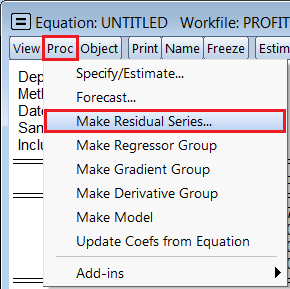
\includegraphics{q1_2}
\end{figure}
\vspace{-\baselineskip}
\begin{figure}[H]
	\centering
	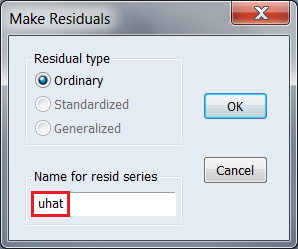
\includegraphics{q1_3}
\end{figure}
\vspace{-\baselineskip}

\noindent To plot the OLS residuals against $ng$ (residual plot),
$$Quick \to Graph \to ng\ resid01 \to Specific:Scatter \to OK$$
\begin{figure}[H]
	\centering
	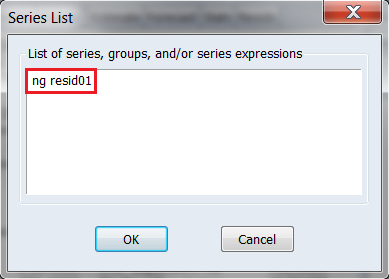
\includegraphics{q1_4}
\end{figure}
\vspace{-\baselineskip}
\begin{figure}[H]
	\centering
	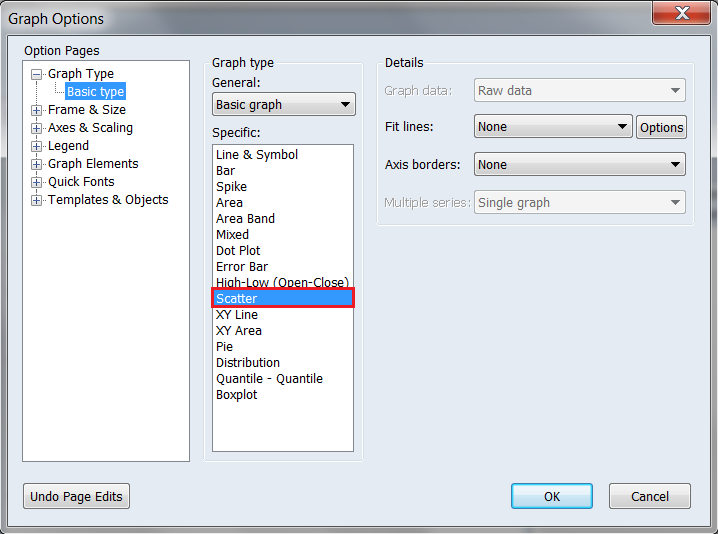
\includegraphics{q1_5}
\end{figure}
\vspace{-\baselineskip}
\begin{figure}[H]
	\centering
	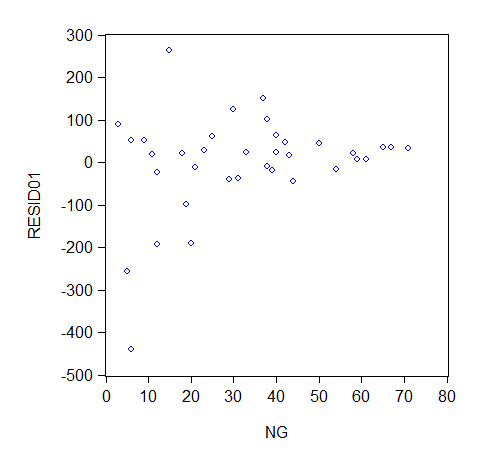
\includegraphics{q1_6}
\end{figure}
\vspace{-\baselineskip}

\newpage
\justify
\begin{blueframed}
	\textcolor{blue}{\textbf{Background}}
	\vspace{-\baselineskip}
	\justify
	\textcolor{blue}{\underline{Breusch-Pagan test for heteroskedasticity}}
	
	\noindent \textcolor{blue}
	{
		\noindent Since $E(u_i|inc_i,nf_i)=0$, 
		\begin{align*}
		Var(u_i|inc_i,nf_i) &= E(u^2_i|inc_i,nf_i) - (E(u_i|inc_i,nf_i))^2 \\
		&= E(u^2_i|inc_i,nf_i)
		\end{align*}
		\noindent we can think about a possible `model' for the $Var(u_i|inc_i,nf_i)$ i.e. one that contains variables that helps to explain $Var(u_i|inc_i,nf_i)$. \\ \\ By considering a model of the squared error term from our model of average food expenditure $u_i = food_i - (\beta_0 + \beta_1 inc_i + \beta_2 nf_i)$, 
		\begin{align*}
		u^2_i &= \delta_0 + \delta_1z_{i1} + \delta_2z_{i2} + \dots + \delta_qz_{iq} + v_i \\
		&= E(u^2_i|z_{i1},z_{i2},\dots,z_{iq}) + v_i \\ 
		&= Var(u_i|z_{i1},z_{i2},\dots,z_{iq}) + v_i
		\end{align*} we see that it is easy to perform a test to see if at least one of the $z$ variables helps to explain the variance of the error.
		\\ \\ Consider $z$ to be a variable of any function of the $x$ variables in our model \textbf{or} any other variable that we have data on which we think can help to explain $Var(food_i|inc_i,nf_i)$ i.e. $Var(u_i|inc_i,nf_i)$ (so the $z$ variables do not have to be $inc$ and $nf$). That is, $$Var(u_i|inc_i,nf_i) = \delta_0 + \delta_1z_{i1} + \delta_2z_{i2} + \dots + \delta_qz_{iq}$$
		\noindent Ideally, we would want to run a regression on,
		\begin{align*}
		u^2_i &= \delta_0 + \delta_1z_{i1} + \delta_2z_{i2} + \dots + \delta_qz_{iq} + v_i \\
		&= E(u^2_i|inc_i,nf_i) + v_i \\
		&= Var(u_i|inc_i,nf_i) + v_i
		\end{align*}
		\noindent and test for heteroskedasticity by testing if at least one of the $z$ variables has any explanatory power in explaining the variance of $u$ (and therefore the variance of $food$), $$H_1: at\ least\ one\ of\ \delta_j\ does\ not\ equal\ 0\ \quad for\ j=1,2,\dots,q$$ but this is not feasible because we do not observe $u^2$ so we cannot run the regression.
		\\ \\ What we do is replace $u$ with the observable OLS residuals $\hat{u}$,
		$$\hat{u}^2_i = \delta_0 + \delta_1z_{i1} + \delta_2z_{i2} + \dots + \delta_qz_{iq} + v_i$$
	}
\end{blueframed}

\justify
\begin{blueframed}
	\vspace{-\baselineskip}
	\justify
	\noindent \textcolor{blue}
	{	\noindent run this \textit{auxiliary regression}, 
		$$Quick \to Estimate\ Equation \to \dots$$
		\noindent then test if at least one of the $z$ variables has explanatory power in explaining the variance of $u$,
		\begin{align*}
		&H_0: \delta_1 = \delta_2 = \dots = \delta_q = 0 \\
		&H_1:at\ least\ one\ of\ the\ above\ \delta_i \neq 0\ for\ i=1,2,..,q
		\end{align*}
		For the general case of $q$, $z$ variables, so we would formulate the null and alternative hypothesis as follows, $$Var(u_i|inc_i,nf_i) = E(u^2_i|inc_i,nf_i) = \delta_0 + \delta_1z_{i1} + \delta_2z_{i2} + \dots + \delta_qz_{iq}$$
		\begin{align*}
		&H_0: E(u^2_i|inc_i,nf_i) = \sigma^2 \quad (\delta_1 = \delta_2 = \dots = \delta_q = 0 \quad homoskedastic\ errors) \\
		&H_1: E(u^2_i|inc_i,nf_i) \neq \sigma^2 \quad (at\ least\ one\ of\ the\ above\ \delta's \neq 0 \quad heteroskedastic\ errors)
		\end{align*} ($\sigma^2$ and $\delta$ are constants)
	}
\end{blueframed}

\noindent Using our intuition and visual aid, we suspect that $ng_i$ has an inverse relationship with $Var(u_i|inc_i,nf_i)$, therefore, we let $\dfrac{1}{ng_i}$ be a variable in our \textbf{auxiliary regression},

$$\hat{u}^2_i = \delta_0 + \delta_1\dfrac{1}{ng_i} + v_i$$

\noindent (If we suspect that there are other variables that affect the variance of the error and we have data on these variables, we should include them in the auxiliary regression when testing for heteroskedasticity in the error using Breusch-Pagan test.)

\noindent $H_0: E(u^2_i|inc_i,nf_i) = \sigma^2 \qquad (\delta_1 = 0 \quad homoskedastic\ errors)$

\noindent $H_1: E(u^2_i|inc_i,nf_i) \neq \sigma^2 \qquad (\delta_1 \neq 0 \quad heteroskedastic\ errors)$

\noindent The Breusch-Pagan test statistic,
$$LM =  N\times R^2_{aux} \sim \chi_{q}^2$$ $$R^2_{aux}: R^2\ from\ the\ auxiliary\ regression$$ $$q:number\ of\ regressors\ in\ the\ auxiliary\ regression$$
\noindent where $q$ represents the number of variables which we believe impact the variance of the error and are include as regressors in the auxiliary regression of the Breusch-Pagan test.

\noindent To estimate the auxiliary regression in EViews,
\begin{figure}[H]
	\centering
	
\includegraphics{tute10_1}
\end{figure}
\vspace{-\baselineskip}
%%%%%%%%%% TABLE OBJECT %%%%%%%%%%
\begin{table}[H]
	\centering
	\begin{tabular}{lrrrr}
		\multicolumn{3}{l}{Dependent Variable: RESID01\textasciicircum 2}&\multicolumn{1}{c}{}&\multicolumn{1}{c}{}\\
		\multicolumn{3}{l}{Method: Least Squares}&\multicolumn{1}{c}{}&\multicolumn{1}{c}{}\\
		\multicolumn{3}{l}{Date: 05/06/18   Time: 19:16}&\multicolumn{1}{c}{}&\multicolumn{1}{c}{}\\
		\multicolumn{2}{l}{Sample: 1 37}&\multicolumn{1}{c}{}&\multicolumn{1}{c}{}&\multicolumn{1}{c}{}\\
		\multicolumn{3}{l}{Included observations: 37}&\multicolumn{1}{c}{}&\multicolumn{1}{c}{}\\
		[4.5pt] \hline \\ [-4.5pt]
		\multicolumn{1}{c}{Variable}&\multicolumn{1}{r}{Coefficient}&\multicolumn{1}{r}{Std. Error}&\multicolumn{1}{r}{t-Statistic}&\multicolumn{1}{r}{Prob.}\\
		[4.5pt] \hline \\ [-4.5pt]
		\multicolumn{1}{c}{C}&\multicolumn{1}{r}{$1372.979$}&\multicolumn{1}{r}{$7123.362$}&\multicolumn{1}{r}{$0.192743$}&\multicolumn{1}{r}{$0.8483$}\\
		\multicolumn{1}{c}{1/NG}&\multicolumn{1}{r}{$212500.3$}&\multicolumn{1}{r}{$82855.09$}&\multicolumn{1}{r}{$2.564722$}&\multicolumn{1}{r}{$0.0148$}\\
		[4.5pt] \hline \\ [-4.5pt]
		\multicolumn{1}{l}{R-squared}&\multicolumn{1}{r}{$0.158205$}&\multicolumn{2}{l}{Mean dependent var}&\multicolumn{1}{r}{$13550.23$}\\
		\multicolumn{1}{l}{Adjusted R-squared}&\multicolumn{1}{r}{$0.134153$}&\multicolumn{2}{l}{S.D. dependent var}&\multicolumn{1}{r}{$34713.39$}\\
		\multicolumn{1}{l}{S.E. of regression}&\multicolumn{1}{r}{$32301.11$}&\multicolumn{2}{l}{Akaike info criterion}&\multicolumn{1}{r}{$23.65613$}\\
		\multicolumn{1}{l}{Sum squared resid}&\multicolumn{1}{r}{$3.65E+10$}&\multicolumn{2}{l}{Schwarz criterion}&\multicolumn{1}{r}{$23.74321$}\\
		\multicolumn{1}{l}{Log likelihood}&\multicolumn{1}{r}{$-435.6384$}&\multicolumn{2}{l}{Hannan-Quinn criter.}&\multicolumn{1}{r}{$23.68683$}\\
		\multicolumn{1}{l}{F-statistic}&\multicolumn{1}{r}{$6.577799$}&\multicolumn{2}{l}{Durbin-Watson stat}&\multicolumn{1}{r}{$2.379673$}\\
		\multicolumn{1}{l}{Prob(F-statistic)}&\multicolumn{1}{r}{$0.014773$}&\multicolumn{1}{c}{}&\multicolumn{1}{c}{}&\multicolumn{1}{c}{}\\
		[4.5pt] \hline \\ [-4.5pt]
	\end{tabular}
	%\caption{Add your caption here.}
	%\label{tab:}
\end{table}

\centering $LM_{calc} = 37 \times 0.158205 = 5.8534$ 

\justify \noindent To obtain the critical value in EViews,
\begin{figure}[H]
	\centering
	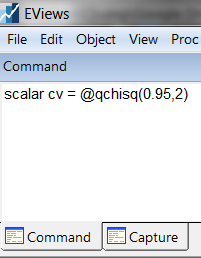
\includegraphics{tute10_2}
\end{figure}
\vspace{-\baselineskip}
\begin{figure}[H]
	\centering
	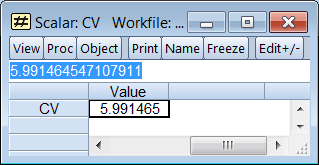
\includegraphics{tute10_3}
\end{figure}
\vspace{-\baselineskip}

\noindent Since $LM_{calc} = 5.8534 > \chi^2_{crit} = 3.8415$, we reject $H_0$ at the 5\% significance level and conclude that there is sufficient evidence from our sample to suggest that the errors are heteroskedastic.

\noindent Note: This test is only valid for larger samples, so our conclusion should be taken with consideration to the sample size and used in conjunction with theoretical reasoning and our visual findings. 

\newpage
\noindent EViews has an inbuilt Breusch-Pagan (and White test) for heteroskedasticity which you can use to verify your results,
$$After\ you\ estimate\ your\ model\ with\ OLS$$
$$From\ the\ equation\ object:$$
$$View \to Residual\ Diagnostics \to Heteroskedasticity\ Tests... $$
\begin{figure}[H]
	\centering
	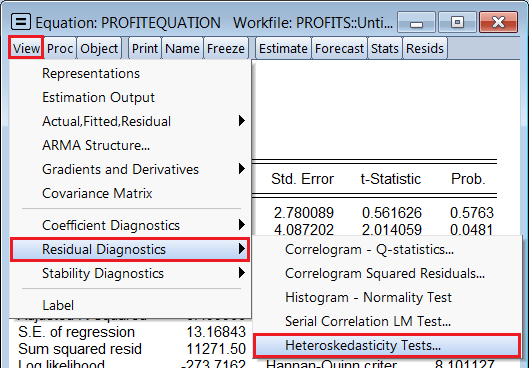
\includegraphics{tute10_6}
\end{figure}
\vspace{-\baselineskip}
\begin{figure}[H]
	\centering
	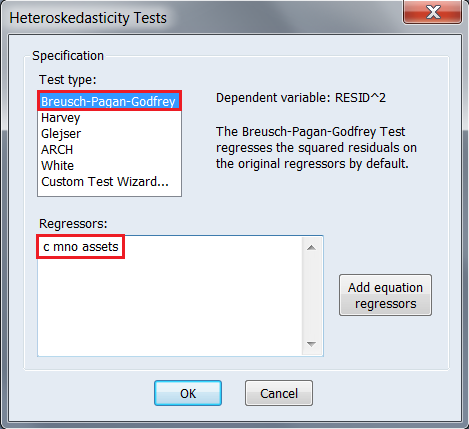
\includegraphics{q1_8}
\end{figure}
\vspace{-\baselineskip}
$$\textbf{Test}\ \textbf{type}: Breusch-Pagan-Godfrey$$
$$\textbf{Regressors}: c \quad 1/ng$$
%%%%%%%%%% TABLE OBJECT %%%%%%%%%%
\begin{table}[H]
	\centering
	\begin{tabular}{lrrrr}
		\multicolumn{5}{l}{Heteroskedasticity Test: Breusch-Pagan-Godfrey}\\
		[4.5pt] \hline \\ [-4.5pt]
		\multicolumn{1}{l}{F-statistic}&\multicolumn{1}{r}{$6.577799$}&\multicolumn{2}{l}{Prob. F(1,35)}&\multicolumn{1}{r}{$0.0148$}\\
		\multicolumn{1}{l}{Obs*R-squared}&\multicolumn{1}{r}{$5.853570$}&\multicolumn{2}{l}{Prob. Chi-Square(1)}&\multicolumn{1}{r}{$0.0155$}\\
		\multicolumn{1}{l}{Scaled explained SS}&\multicolumn{1}{r}{$15.78144$}&\multicolumn{2}{l}{Prob. Chi-Square(1)}&\multicolumn{1}{r}{$0.0001$}\\
		[4.5pt] \hline \\ [-4.5pt]
		\multicolumn{1}{c}{}&\multicolumn{1}{c}{}&\multicolumn{1}{c}{}&\multicolumn{1}{c}{}&\multicolumn{1}{c}{}\\
		\multicolumn{2}{l}{Test Equation:}&\multicolumn{1}{c}{}&\multicolumn{1}{c}{}&\multicolumn{1}{c}{}\\
		\multicolumn{3}{l}{Dependent Variable: RESID\textasciicircum 2}&\multicolumn{1}{c}{}&\multicolumn{1}{c}{}\\
		\multicolumn{3}{l}{Method: Least Squares}&\multicolumn{1}{c}{}&\multicolumn{1}{c}{}\\
		\multicolumn{3}{l}{Date: 05/08/18   Time: 18:09}&\multicolumn{1}{c}{}&\multicolumn{1}{c}{}\\
		\multicolumn{2}{l}{Sample: 1 37}&\multicolumn{1}{c}{}&\multicolumn{1}{c}{}&\multicolumn{1}{c}{}\\
		\multicolumn{3}{l}{Included observations: 37}&\multicolumn{1}{c}{}&\multicolumn{1}{c}{}\\
		[4.5pt] \hline \\ [-4.5pt]
		\multicolumn{1}{c}{Variable}&\multicolumn{1}{r}{Coefficient}&\multicolumn{1}{r}{Std. Error}&\multicolumn{1}{r}{t-Statistic}&\multicolumn{1}{r}{Prob.}\\
		[4.5pt] \hline \\ [-4.5pt]
		\multicolumn{1}{c}{C}&\multicolumn{1}{r}{$1372.979$}&\multicolumn{1}{r}{$7123.362$}&\multicolumn{1}{r}{$0.192743$}&\multicolumn{1}{r}{$0.8483$}\\
		\multicolumn{1}{c}{1/NG}&\multicolumn{1}{r}{$212500.3$}&\multicolumn{1}{r}{$82855.09$}&\multicolumn{1}{r}{$2.564722$}&\multicolumn{1}{r}{$0.0148$}\\
		[4.5pt] \hline \\ [-4.5pt]
		\multicolumn{1}{l}{R-squared}&\multicolumn{1}{r}{$0.158205$}&\multicolumn{2}{l}{Mean dependent var}&\multicolumn{1}{r}{$13550.23$}\\
		\multicolumn{1}{l}{Adjusted R-squared}&\multicolumn{1}{r}{$0.134153$}&\multicolumn{2}{l}{S.D. dependent var}&\multicolumn{1}{r}{$34713.39$}\\
		\multicolumn{1}{l}{S.E. of regression}&\multicolumn{1}{r}{$32301.11$}&\multicolumn{2}{l}{Akaike info criterion}&\multicolumn{1}{r}{$23.65613$}\\
		\multicolumn{1}{l}{Sum squared resid}&\multicolumn{1}{r}{$3.65E+10$}&\multicolumn{2}{l}{Schwarz criterion}&\multicolumn{1}{r}{$23.74321$}\\
		\multicolumn{1}{l}{Log likelihood}&\multicolumn{1}{r}{$-435.6384$}&\multicolumn{2}{l}{Hannan-Quinn criter.}&\multicolumn{1}{r}{$23.68683$}\\
		\multicolumn{1}{l}{F-statistic}&\multicolumn{1}{r}{$6.577799$}&\multicolumn{2}{l}{Durbin-Watson stat}&\multicolumn{1}{r}{$2.379673$}\\
		\multicolumn{1}{l}{Prob(F-statistic)}&\multicolumn{1}{r}{$0.014773$}&\multicolumn{1}{c}{}&\multicolumn{1}{c}{}&\multicolumn{1}{c}{}\\
		[4.5pt] \hline \\ [-4.5pt]
	\end{tabular}
	%\caption{Add your caption here.}
	%\label{tab:}
\end{table} \centering
$LM_{calc} = 5.8536 \qquad p-value=0.0155$


\newpage
\justify
\noindent \textcolor{red}
{
	(d) Suppose we reject homoskedasticity in favour of,
	$$Var(u_i|inc_i,nf_i)=\dfrac{\sigma^2}{ng_i}$$
	Describe how we should transform the variables and which regression we should run to obtain the best linear unbiased estimator for $\beta_0$, $\beta_1$ and $\beta_2$.
}

\justify
\begin{blueframed}
	\textcolor{blue}{\textbf{Background}}
	\vspace{-\baselineskip}
	\justify
	\textcolor{blue}{\underline{Weighted Least Squares Estimator}}
	
	\noindent \textcolor{blue}
	{
		\noindent It is helpful to consider the WLS estimator as a 2-step estimator: \begin{itemize}
			\item At step 1, apply some weighting/transformation to the original model to obtain the weighted model.
			\item At step 2, estimate the weighted model by OLS.
		\end{itemize} If the variance of the error has the following known functional form,
		$$Var(u_i|x_{i1},x_{i2},...) = \sigma^2h_i$$
		\noindent then weighing the original model by,
		$$w_i = \dfrac{1}{\sqrt{h_i}}$$
		\noindent produces the following weighted model, $$w_iy_i = \beta_0w_i + \beta_1w_ix_{i1} + \beta_2w_ix_{i2} + \dots + w_iu_i$$ with a constant error variance 		(homoskedastic error),
		\begin{align*}
		Var(w_iu_i|x_{i1},x_{i2},\dots) &= w^2_iVar(u_i|x_{i1},x_{i2},\dots) \\
		&= \dfrac{1}{h_i}Var(u_i|x_{i1},x_{i2},\dots) \\
		&= \dfrac{1}{h_i}\sigma^2h_i \\
		&= \sigma^2
		\end{align*}
		The weight, $w_i$, is known and not treated a random variable. \\ \\ The Weighted Least Squares (WLS) estimator is the OLS estimator used to estimate the weighted model of $y$ (weighted so that the error has constant variance).
	}
\end{blueframed}

\noindent Since the variance of the error takes the following form,
$$Var(u_i|inc_i,nf_i)=\dfrac{\sigma^2}{ng_i}$$
\noindent then the weight that we need to apply to our original model to obtain a weighted model with constant error variance is given by,
$$w_i = \dfrac{1}{\sqrt{1/ng_i}} = \sqrt{ng_i}$$
\noindent Multiplying $w_i$ on both sides of the original model of $food_i$ gives the following weighted model of $food_i$,
$$\sqrt{ng_i}food_i = \beta_0\sqrt{ng_i} + \beta_1\sqrt{ng_i}inc_i + \beta_2\sqrt{ng_i}nf_i + \sqrt{ng_i}u_i$$
\noindent and the error term in this weighted model has constant variance,
\begin{align*}
Var(\sqrt{ng_i}u_i|inc_i,nf_i) &= (\sqrt{ng_i})^2Var(u_i|x_{i1},x_{i2},\dots) \\
&= ng_iVar(u_i|x_{i1},x_{i2},\dots) \\
&= ng_i\dfrac{\sigma^2}{ng_i} \\
&= \sigma^2
\end{align*}
\noindent To estimate the weighted model from the \textbf{Command window},
$$ls \quad @sqrt(ng)^*food \quad @sqrt(ng) \quad @sqrt(ng)^*inc \quad @sqrt(ng)^*nf$$
\begin{figure}[H]
	\centering
	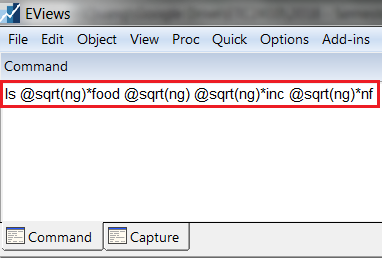
\includegraphics{tute10_4}
\end{figure}
\vspace{-\baselineskip}


%%%%%%%%%% TABLE OBJECT %%%%%%%%%%
\begin{table}[H]
	\centering
	\begin{tabular}{lrrrr}
		\multicolumn{4}{l}{Dependent Variable: @SQRT(NG)*FOOD}&\multicolumn{1}{c}{}\\
		\multicolumn{3}{l}{Method: Least Squares}&\multicolumn{1}{c}{}&\multicolumn{1}{c}{}\\
		\multicolumn{3}{l}{Date: 05/06/18   Time: 19:45}&\multicolumn{1}{c}{}&\multicolumn{1}{c}{}\\
		\multicolumn{2}{l}{Sample: 1 37}&\multicolumn{1}{c}{}&\multicolumn{1}{c}{}&\multicolumn{1}{c}{}\\
		\multicolumn{3}{l}{Included observations: 37}&\multicolumn{1}{c}{}&\multicolumn{1}{c}{}\\
		[4.5pt] \hline \\ [-4.5pt]
		\multicolumn{1}{c}{Variable}&\multicolumn{1}{r}{Coefficient}&\multicolumn{1}{r}{Std. Error}&\multicolumn{1}{r}{t-Statistic}&\multicolumn{1}{r}{Prob.}\\
		[4.5pt] \hline \\ [-4.5pt]
		\multicolumn{1}{c}{@SQRT(NG)}&\multicolumn{1}{r}{$70.31890$}&\multicolumn{1}{r}{$28.51754$}&\multicolumn{1}{r}{$2.465813$}&\multicolumn{1}{r}{$0.0189$}\\
		\multicolumn{1}{c}{@SQRT(NG)*INC}&\multicolumn{1}{r}{$0.177184$}&\multicolumn{1}{r}{$0.010268$}&\multicolumn{1}{r}{$17.25529$}&\multicolumn{1}{r}{$0.0000$}\\
		\multicolumn{1}{c}{@SQRT(NG)*NF}&\multicolumn{1}{r}{$57.70058$}&\multicolumn{1}{r}{$8.056305$}&\multicolumn{1}{r}{$7.162164$}&\multicolumn{1}{r}{$0.0000$}\\
		[4.5pt] \hline \\ [-4.5pt]
	\end{tabular}
	%\caption{Add your caption here.}
	%\label{tab:}
\end{table}

$$\widehat{food}_i = \underset{(28.5175)}{70.3189} + \underset{(0.0103)}{0.1772}inc_i + \underset{(8.0563)}{57.7006}nf_i$$

\noindent This process of applying a transformation to the model is a device for converting a model with heteroskedastic errors into a model with homoskedasticity error. It is NOT something that changes the inherent meaning of the coefficients. As such, we still interpret the ‘weighted’ coefficients and report our results in the same way as we would with the original model.


\noindent \textcolor{red}
{
	(e) Based on the weighted least squares estimates test the hypothesis that, other things staying the same, a 1 dollar increase in family income will result a 20 cent increase in family food consumption, against the alternative that it will result in a less than 20 cent increase in food consumption. Perform this test at the 5\% level of significance.
}
%%%%%%%%%% TABLE OBJECT %%%%%%%%%%
\begin{table}[H]
	\centering
	\begin{tabular}{lrrrr}
		\multicolumn{4}{l}{Dependent Variable: @SQRT(NG)*FOOD}&\multicolumn{1}{c}{}\\
		\multicolumn{3}{l}{Method: Least Squares}&\multicolumn{1}{c}{}&\multicolumn{1}{c}{}\\
		\multicolumn{3}{l}{Date: 05/06/18   Time: 19:45}&\multicolumn{1}{c}{}&\multicolumn{1}{c}{}\\
		\multicolumn{2}{l}{Sample: 1 37}&\multicolumn{1}{c}{}&\multicolumn{1}{c}{}&\multicolumn{1}{c}{}\\
		\multicolumn{3}{l}{Included observations: 37}&\multicolumn{1}{c}{}&\multicolumn{1}{c}{}\\
		[4.5pt] \hline \\ [-4.5pt]
		\multicolumn{1}{c}{Variable}&\multicolumn{1}{r}{Coefficient}&\multicolumn{1}{r}{Std. Error}&\multicolumn{1}{r}{t-Statistic}&\multicolumn{1}{r}{Prob.}\\
		[4.5pt] \hline \\ [-4.5pt]
		\multicolumn{1}{c}{@SQRT(NG)}&\multicolumn{1}{r}{$70.31890$}&\multicolumn{1}{r}{$28.51754$}&\multicolumn{1}{r}{$2.465813$}&\multicolumn{1}{r}{$0.0189$}\\
		\multicolumn{1}{c}{@SQRT(NG)*INC}&\multicolumn{1}{r}{$0.177184$}&\multicolumn{1}{r}{$0.010268$}&\multicolumn{1}{r}{$17.25529$}&\multicolumn{1}{r}{$0.0000$}\\
		\multicolumn{1}{c}{@SQRT(NG)*NF}&\multicolumn{1}{r}{$57.70058$}&\multicolumn{1}{r}{$8.056305$}&\multicolumn{1}{r}{$7.162164$}&\multicolumn{1}{r}{$0.0000$}\\
		[4.5pt] \hline \\ [-4.5pt]
	\end{tabular}
	%\caption{Add your caption here.}
	%\label{tab:}
\end{table}
\centering $\widehat{food}_i = \underset{(28.5175)}{70.3189} + \underset{(0.0103)}{0.1772}inc_i + \underset{(8.0563)}{57.7006}nf_i$
\begin{align*}
&H_0: \beta_1 = 0.2 \\
&H_1: \beta_1 < 0.2
\end{align*}
$$t = \dfrac{\hat{\beta}_1 - \beta_1}{se(\hat{\beta}_1)} = \dfrac{\hat{\beta}_1 - 0.2}{se(\hat{\beta}_1)} \sim t_{n-k-1}\ under\ H_0$$
$t_{calc} = \dfrac{0.1772 - 0.2}{0.0103} = -2.2136$
\begin{figure}[H]
	\centering
	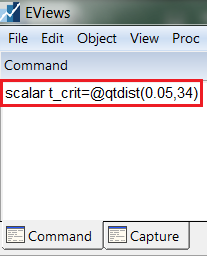
\includegraphics{tute10_5}
\end{figure}
\vspace{-\baselineskip}
$-t_{crit} = t_{34,0.05} = -1.6909$

\justify \noindent Since $t_{calc} = -2.2136 > -t_{crit} = -1.6909$ we reject the null and conclude that there is sufficient evidence from our sample to suggest that a dollar increase in family income will result in a less than 20 cent increase in food consumption, holding $nf$ constant.
\end{document}